%%%%%%%%%%%%%%%%%%%%%%%%%%%%%%%%%%%%%%%%%%%%%%%%%%%%%%%%%%%%%%%%%%%%%%%%%%%%%%%%
%%%%%%%%%%%%%%%%%%   Vorlage für eine Abschlussarbeit   %%%%%%%%%%%%%%%%%%%%%%%%
%%%%%%%%%%%%%%%%%%%%%%%%%%%%%%%%%%%%%%%%%%%%%%%%%%%%%%%%%%%%%%%%%%%%%%%%%%%%%%%%

% Erstellt von Maximilian Nöthe, <maximilian.noethe@tu-dortmund.de>
% ausgelegt für lualatex und Biblatex mit biber

% Kompilieren mit
% latexmk --lualatex --output-directory=build thesis.tex
% oder einfach mit:
% make

\documentclass[
  tucolor,       % remove for less green,
  BCOR=12mm,     % 12mm binding corrections, adjust to fit your binding
  parskip=half,  % new paragraphs start with half line vertical space
  open=any,      % chapters start on both odd and even pages
  cleardoublepage=plain,  % no header/footer on blank pages
]{tudothesis}


% Warning, if another latex run is needed
\usepackage[aux]{rerunfilecheck}

% just list chapters and sections in the toc, not subsections or smaller
% \setcounter{tocdepth}{1}
% MODIFIED: We apply this only to the rendered TOC,
% so that the TOC embedded in the PDF still contains subsections.

%------------------------------------------------------------------------------
%------------------------------ Fonts, Unicode, Language ----------------------
%------------------------------------------------------------------------------
\usepackage{fontspec}
\defaultfontfeatures{Ligatures=TeX}  % -- becomes en-dash etc.

% load english (for abstract) and ngerman language
% the main language has to come last
\usepackage[ngerman, american]{babel}

% intelligent quotation marks, language and nesting sensitive
\usepackage[autostyle]{csquotes}

% microtypographical features, makes the text look nicer on the small scale
\usepackage{microtype}

%------------------------------------------------------------------------------
%------------------------ Math Packages and settings --------------------------
%------------------------------------------------------------------------------

\usepackage{amsmath}
\usepackage{amssymb}
\usepackage{mathtools}

% Enable Unicode-Math and follow the ISO-Standards for typesetting math
\usepackage[
  math-style=ISO,
  bold-style=ISO,
  sans-style=italic,
  nabla=upright,
  partial=upright,
]{unicode-math}
\setmathfont{Latin Modern Math}

% nice, small fracs for the text with \sfrac{}{}
\usepackage{xfrac}


%------------------------------------------------------------------------------
%---------------------------- Numbers and Units -------------------------------
%------------------------------------------------------------------------------

\usepackage[
  locale=US,
  separate-uncertainty=true,
  per-mode=symbol-or-fraction,
]{siunitx}
\sisetup{math-micro=\text{µ},text-micro=µ}

%------------------------------------------------------------------------------
%-------------------------------- tables  -------------------------------------
%------------------------------------------------------------------------------

\usepackage{booktabs}       % \toprule, \midrule, \bottomrule, etc

%------------------------------------------------------------------------------
%-------------------------------- graphics -------------------------------------
%------------------------------------------------------------------------------

\usepackage{graphicx}
% currently broken
% \usepackage{grffile}

% allow figures to be placed in the running text by default:
\usepackage{scrhack}
\usepackage{float}
\floatplacement{figure}{htbp}
\floatplacement{table}{htbp}

% keep figures and tables in the section
\usepackage[section, below]{placeins}


%------------------------------------------------------------------------------
%---------------------- customize list environments ---------------------------
%------------------------------------------------------------------------------

\usepackage{enumitem}

%------------------------------------------------------------------------------
%------------------------------ Bibliographie ---------------------------------
%------------------------------------------------------------------------------

\usepackage[
  backend=biber,   % use modern biber backend
  autolang=hyphen, % load hyphenation rules for if language of bibentry is not
                   % german, has to be loaded with \setotherlanguages
                   % in the references.bib use langid={en} for english sources
]{biblatex}
\addbibresource{references.bib}  % the bib file to use
\DefineBibliographyStrings{american}{andothers = {{et\,al\adddot}}}  % replace u.a. with et al.


% Last packages, do not change order or insert new packages after these ones
\usepackage[pdfusetitle, unicode, linkbordercolor=tugreen, citebordercolor=tugreen]{hyperref}
\usepackage{bookmark}
\usepackage[shortcuts]{extdash}

%------------------------------------------------------------------------------
%------------------------------ Custom dependencies ---------------------------
%------------------------------------------------------------------------------

\usepackage[nolist,nohyperlinks]{acronym}
\usepackage{blindtext}
\usepackage{todonotes}
\usepackage[outputdir=build]{minted}
\usepackage[nameinlink]{cleveref}
\usepackage{pdfpages}

\usepackage{algorithm}
\usepackage{algpseudocode}
\renewcommand{\algorithmicrequire}{\textbf{Input:}}
\renewcommand{\algorithmicensure}{\textbf{Output:}}

%------------------------------------------------------------------------------
%------------------------------ Custom commands -------------------------------
%------------------------------------------------------------------------------


% █ Acronyms/… → managed by the acronym package
% ▒ IceCube things
\acrodef{DOM}{digital optical module}
\acrodef{PMT}{photomultiplier tube}
% ▒ Algorithms
% {acronym} [short name] {full name}
\acrodef{Adam}{Adaptive Moment Estimation}
\acrodef{CORN}{\textbf{C}onditional \textbf{O}rdinal \textbf{R}egression for \textbf{N}eural Networks}
\acrodef{CORAL}{\textbf{CO}onsistent \textbf{RA}ank \textbf{L}ogits}
\acrodef{DSEANONPLUS}[DSEA]{Dortmund Spectrum Estimation Algorithm}
\acused{DSEANONPLUS} % never print the full name
\acrodef{DSEAPLUS}[DSEA\textsuperscript{+}]{Dortmund Spectrum Estimation Algorithm}
\acrodef{TRUEE}{Time-dependent Regularized Unfolding for Economics and Engineerings}
\acrodef{RUN}{Regularized Unfolding}
\acrodef{IBU}{Iterative Bayesian Unfolding}
% ▒ Metrics
\acrodef{MAE}{mean absolute error}
\acrodef{RMSE}{root mean squared error}
\acrodef{EMD}{earth mover's distance}
\acrodef{WD}{Wasserstein distance}

% █ Acronyms/… → custom
% ▒ Misc.
\newcommand{\icecube}{IceCube}
% ▒ DSEA versions → regular
% NOTE: These aren't used for section titles, since their font does not support textsc.
\newcommand{\dseanonplus}{\ac{DSEANONPLUS}}
\newcommand{\dseaplus}{\ac{DSEAPLUS}}
\newcommand{\dsea}{\dseaplus{}} % default to DSEA+
% ▒ DSEA versions → title
\newcommand{\dseanonplustitle}{DSEA}
\newcommand{\dseaplustitle}{\texorpdfstring{DSEA\textsuperscript{+}}{DSEA+}}
\newcommand{\dseatitle}{\dseaplustitle{}} % default to DSEA+

% █ Names/…
\newcommand{\icecubeneutrinoobservatory}{\icecube{} Neutrino Observatory}

% ▒ Wikipedia-style "citation needed" macro
% https://gist.github.com/martinarroyo/b9e0a963ad27169a6eee?permalink_comment_id=2355734#gistcomment-2355734
\newcommand{\citationneeded}{\textsuperscript{\color{blue} [citation needed]}}

%------------------------------------------------------------------------------
%-------------------------    Angaben zur Arbeit   ----------------------------
%------------------------------------------------------------------------------

\author{Nicolai Weitkemper}
% ↓ NOTE: Technically, it's DSEA+, but it's already registered this way.
\title{Ordinal Classification with Neural Networks in DSEA}
\date{2022}
\birthplace{Soest}
\chair{Lehrstuhl für Experimentelle Physik V}
\division{Fakultät Physik}
\thesisclass{Bachelor of Science}
\submissiondate{30. September 2022}
\firstcorrector{Prof.~Dr.~Dr.~Wolfgang~Rhode}
\secondcorrector{Prof.~Dr.~Johannes~Albrecht}

% tu logo on top of the titlepage
\titlehead{
\includegraphics[height=1.5cm]{logos/tu-logo.pdf}}

\begin{document}
  \frontmatter
  \maketitle

  % Gutachterseite
  \makecorrectorpage

  % hier beginnt der Vorspann, nummeriert in römischen Zahlen
  \thispagestyle{plain}

\section*{Abstract}
% - Neutrinos
% - IceCube
% - DSEA
% - CORN
% - THIS THESIS

The deconvolution of energy spectra is a [common] problem in neutrino astronomy.
As an inverse problem,
  it requires special methods to solve.
The \textbf{D}ortmund \textbf{S}pectrum \textbf{E}stimation \textbf{A}lgorithm (\dsea{}) \cite{dsea_unification}
solves the deconvolution problem
  by using a classifier to estimate the discretized energy spectrum
  and iteratively reweighting the training data.
%
In the given problem,
  neutrino energies are \emph{ordinal} quantities,
    which means that the order of the energies is important. % COPILOT
However,
  most classifiers do not respect this property.
%
% NOTE: Duplicate of introduction.tex
Previous works
have focused either
  on respecting ordinality \cite{dsea_jan}
  or on using a neural network as a classifier \cite{dsea_samuel}.
This thesis aims to combine the advantages of both approaches:
  the flexibility of neural networks
  and the potential improvements in physical plausibility
    due to respecting ordinality.
The \ac{CORN} framework,
  which [provides] ordinal neural networks,
is adapted to work with \dsea{}
and optimized and evaluated on simulated data from \icecube{}.



\section*{Kurzfassung}
\begin{foreignlanguage}{german}
Hier steht eine Kurzfassung der Arbeit in deutscher Sprache inklusive der Zusammenfassung der
Ergebnisse.
Zusammen mit der englischen Zusammenfassung muss sie auf diese Seite passen.

\blindtext[1]
\end{foreignlanguage}

  \setcounter{tocdepth}{1}
  \tableofcontents
  \setcounter{tocdepth}{2}

  \mainmatter
  % Hier beginnt der Inhalt mit Seite 1 in arabischen Ziffern
  \chapter{Introduction}
% █ astroparticle physics
Astroparticle physics is a relatively new field of physics
  that explores the universe
    with the help of messenger particles.
They carry information about
    the processes that produced them
    and the environment they were created in,
  which can be obtained upon their detection.
% This way, AGN, supernovae, and other astrophysical phenomena can be studied.
% █ neutrino astronomy
Neutrinos are especially valuable messenger particles
  because their propagation path is not affected by electromagnetic fields,
  and they can travel long distances without interacting with matter.
% Therefore,
%   both their source and their energy can be determined
%   by measuring the direction and energy of
%   decay products that they produce in the detector on Earth.

% The most common messenger particles are neutrinos,
% Many high-energy processes are assumed to produce neutrinos.

% █ IceCube
\icecube{} is such a detector,
  which is located at the South Pole.
% ↓ move to icecube.tex?
It makes use of the Antarctic ice as detector material
  and is sensitive to high-energy neutrinos
    in the approximate range of \si{\tera\electronvolt} to \si{\peta\electronvolt} \cite{icecube_aartsen}.
      % \SI{E7}{\electronvolt} to \SI{E21}{\electronvolt}. % source?
%
One goal of analyses with \icecube{} is
  to obtain a neutrino energy spectrum.

% █ DSEA
The \textbf{D}ortmund \textbf{S}pectrum \textbf{E}stimation \textbf{A}lgorithm (\dsea{}) \cite{dsea_unification}
is a method to reconstruct the neutrino energy spectrum
  from the measured data of \icecube{}.
While [conventional] classifiers % TODO
  such as random forests
have been successfully applied to \icecube{} data in \dsea{},
the possibilities of neural networks and deep learning are still largely unexplored. % Naja…
%
Previous works
% that perform unfolding…
have focused either
  on respecting ordinality \cite{dsea_jan} % TODO: Can I explain ordinality here?
  or on using a neural network as a classifier \cite{dsea_samuel}.
This thesis aims to combine the advantages of both approaches:
  the flexibility of neural networks
  and the potential improvements in physical plausibility
    due to respecting ordinality.
% █ CORN
This is done by adapting the
\corn{} (\textbf{C}onditional \textbf{O}rdinal \textbf{R}egression for \textbf{N}eural Networks) framework \cite{corn}
to \dsea{}.
The proposed method is then optimized and evaluated
  on simulated data from \icecube{}.

% █ structure
\Cref{sec:neutrino_astronomy} briefly introduces \icecube{} and important concepts of neutrino astronomy.
\Cref{sec:dsea} describes the deconvolution problem and the \dsea{} approach to solving it.
\Cref{sec:ordinal} [rationalizes/justifies] the need for ordinal classification and introduces the \corn{} framework.
\Cref{sec:unfolding} describes the setup for hyperparameter searches and evaluates the performance of the resulting model. % TODO
\Cref{sec:summary} concludes the thesis and discusses future work.

\chapter{Neutrino Astronomy} \label{sec:neutrino_astronomy}
  This chapter provides
  an introduction to the field of neutrino astronomy
  and describes the \icecube{} neutrino observatory,
    the experimental background of this thesis.

  \section{Neutrinos}

% █ What are neutrinos? What is neutrino astronomy?
Neutrinos are elementary particles with no electric charge and small mass. % [very] small mass…
Their low interactivity
  makes them difficult to detect,
  but is also the reason why they are valuable messenger particles for astroparticle physics:
Since they are not affected by the electromagnetic force,
% and very little by gravity,
  cosmic magnetic fields have no effect on their propagation paths \cite{neutrinos_katz};
  neither does the interstellar medium absorb them in significant amounts.
Together with the energy of the neutrino,
  the direction of propagation % / this information
  is used to determine the location and properties of the source \cite{neutrinos_katz}.


% █ Sources
Neutrinos have various astronomical sources,
  many of which are not experimentally confirmed yet.
This includes
  the \ac{CNB} \cite{follin2015}
     which originates from the Big Bang
  as well as various sources for cosmic ray acceleration
    (and therefore neutrino emission)
  \cite{neutrinos_aartsen_sources},
  such as
    \ac{SNR} shocks,
    \acp{AGN},
    jets,
    starburst galaxies, % Oxford comma
    and gamma-ray bursts.
Neutrinos are also produced in
  the Sun
  and in the Earth's atmosphere % due to cosmic rays!
  as well as in nuclear reactors.
They cover a vast range of energies, from \si{\micro\electronvolt} up to \si{\peta\electronvolt},
  depending on the source. \citationneeded{}
\autoref{fig:neutrinos:flux_spectrum} shows the flux spectrum of neutrinos from different sources.

\begin{figure}
  \centering
  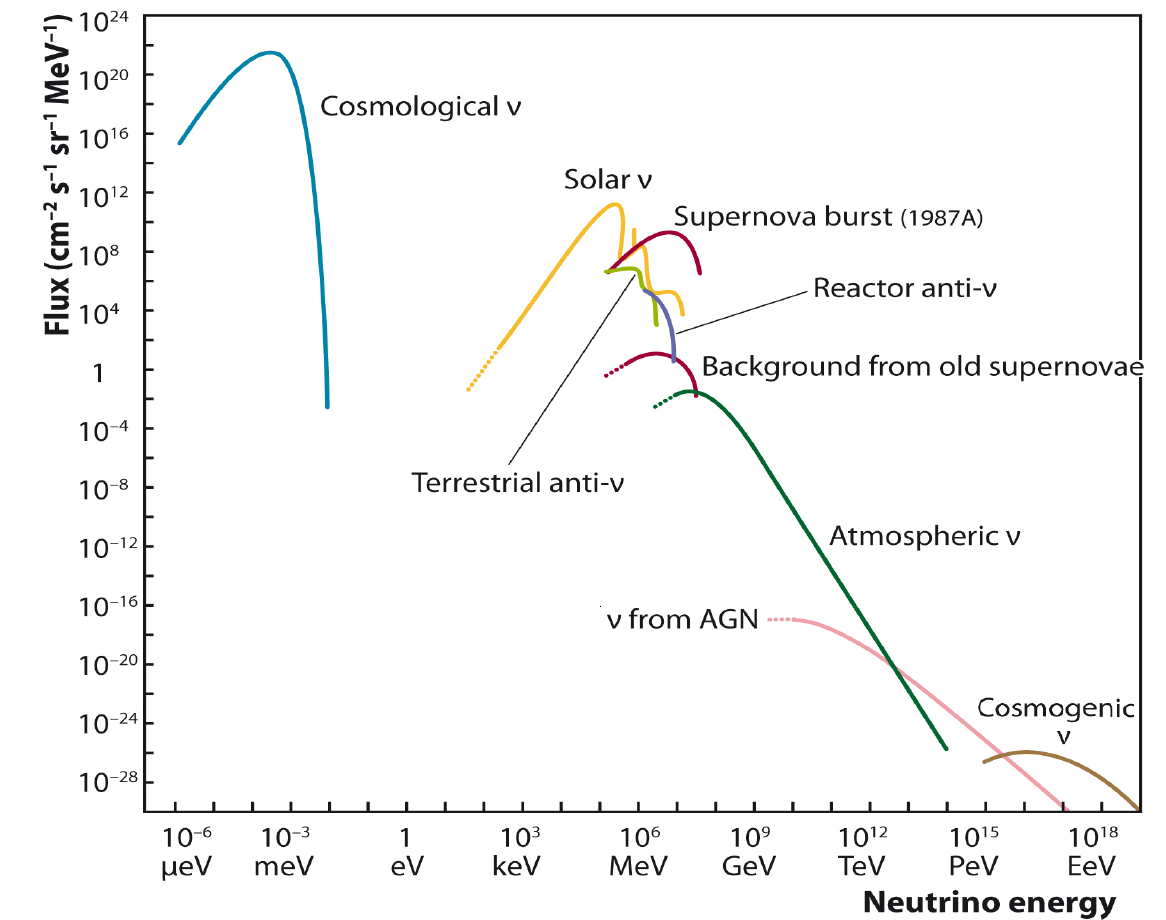
\includegraphics[width=0.75\textwidth]{content/img/neutrino_spectrum.png}
  \caption{
    Measured and expected fluxes of natural and reactor neutrinos as a function of their energy \cite{spiering2012}.
  }
  \label{fig:neutrinos:flux_spectrum}
\end{figure}


% █ Neutrino oscillations
While current models of astrophysical neutrino sources predict a flavor ratio of
  $\phi(\nu_e) : \phi(\nu_\mu) : \phi(\nu_\tau) = 1 : 2 : 0$
    (assuming charged pions decays are the dominant mechanism for neutrino production),
the observed ratio on Earth is
  $1 : 1 : 1$ \cite{neutrinos_beacom}.
This discrepancy is explained by neutrino oscillations \cite{neutrinos_beacom},
  which are a consequence of the fact that neutrinos have mass.
Albeit being very light
  (the current lowest upper limit on the Majorana mass being \qtyrange{0.06}{0.161}{\electronvolt} \cite{neutrinos_gando}),
  it allows for oscillations between the different flavors,
    given the large distances that cosmic neutrinos travel.

  \section{\icecube{}}
The \icecubeneutrinoobservatory{} is located close to the geographic South Pole
  in proximity to the Amundsen-Scott South Pole Station.
% █ Why the South Pole?
It utilizes the optically clear Antarctic ice as detector material,
  with a total detector volume of \SI{1}{\cubic\kilo\meter} \cite{icecube_aartsen}.
The detector is composed of \num{86} strings,
  each consisting of \num{60} \acp{DOM},
    which are positioned
      \SI{17}{\meter} apart along the string
      at depths ranging from \SI{1450}{\meter} to \SI{2450}{\meter} below the surface \cite{icecube_aartsen}.
Each of the \num{5160} \acp{DOM} is equipped with a sensitive \ac{PMT},
  which detects the Cherenkov light emitted by charged particles
    that interact with the ice.
%
\autoref{fig:img:icecube} shows a schematic of the \icecube{} detector.

% \icecube{} detects 275 atmospheric neutrinos daily and about 100,000 per year.


\begin{figure}
  \centering
  % COULDDO: I made this pretty small to accommodate for newly added text.
  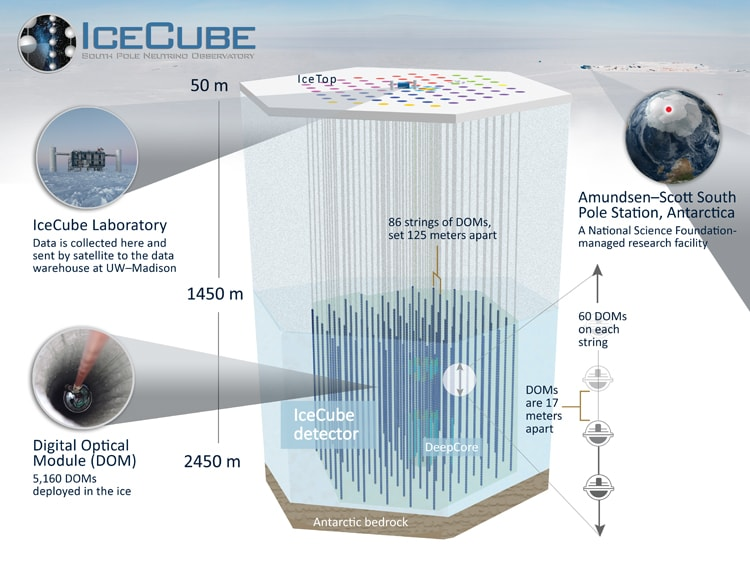
\includegraphics[width=0.65\textwidth]{content/img/icecube_detector_schematic.jpg}
  \caption{
    % Schematic representation
    % Overview
    Infographic
    of the \icecubeneutrinoobservatory{} \cite{icecube_homepage}.
    Each dot represents a \ac{DOM}.
    % COULDDO: longer description
  }
  \label{fig:img:icecube}
\end{figure}


% \subsection{Detection Principle}

% █ Interaction with matter
Neutrinos interact with matter via the weak interaction.
In order to compensate for the low cross-section of the weak interaction,
  the effective detector volume is maximized by utilizing existing naturally occurring detector materials,
  such as
    the Earth's atmosphere,
    the sea,
    or the ice in the Antarctica.
%
When a neutrino interacts with a nucleus in the ice,
it produces a charged lepton and a neutrino.
The charged lepton then produces a Cherenkov light cone
as it propagates through the ice
with greater speed than the speed of light in the ice.
% COULDDO: add Cherenkov figure (in appendix)
The light is detected by the \acp{PMT}
  and
    % (in the case of muon neutrinos, mostly)
  the direction of the neutrino can be reconstructed
    from the position of the \acp{DOM}
      that detected the light.
The intensity of the light and the number of \acp{PMT} that detected it
  are used to determine the energy of the neutrino.
%
\icecube{}
  % (without \emph{DeepCore} and \emph{IceTop})
is sensitive to
  the approximate neutrino energy range
    from \si{\giga\electronvolt} to \si{\peta\electronvolt} \cite{icecube_aartsen}
    % NOTE: “100 GeV for most IceCube analyses” (→ icecube_aartsen)
    % from \SI{E7}{\electronvolt} to \SI{E21}{\electronvolt}. % source: Wikipedia / https://web.archive.org/web/20060909003706/http://icecube.wisc.edu/pub_and_doc/reviews_and_meetings/June2002_NRC-Review/presentations/nrc_halzen.pdf
  and therefore primarily to atmospheric and \ac{AGN} neutrinos.
Higher energies require even larger detector volumes.

Depending on the flavor of the leptons,
different types of interactions occur,
allowing to determine the flavor of the neutrino in turn.
%
% NOTE: The following differentiation is a little hand-wavy.
% For example, ALL neutrino flavors can shower to produce spherical signatures (→ icecube_aartsen).
%
% ▒ µ-neutrinos
% NOTE: The Monte Carlo data used in this work only contains muon neutrinos.
% ORIG[icecube_aartsen]: Track-like events originate from a charged-current interaction of a high-energy muon neutrino with a nucleus, producing a hadronic shower at the vertex and an outgoing muon that emits Cherenkov light in a cone along its track. The angular resolution for muon tracks and hence the incident neutrino direction is typically 0.6°, confirmed by analysis of the shadows of the Moon and Sun in cosmic rays [19, 20]. Muons with energies above a critical energy, about 1 TeV in ice, predominantly lose energy by radiative processes that exhibit a stochastic behavior with large fluctuations. This results in large variability in the amount of energy deposited for different muons of the same energy.
%
Muon neutrinos are detected as \emph{tracks} \cite{icecube_aartsen}
  which originate from a charged-current interaction of a high-energy muon neutrino with a nucleus.
They have a good angular resolution
  because muons typically fall under the Cherenkov limit as soon as they scatter.
%
% ▒ e-neutrinos
% ORIG[Wikipedia]: IceCube is more sensitive to muons than other charged leptons, because they are the most penetrating and thus have the longest tracks in the detector. Thus, of the neutrino flavors, IceCube is most sensitive to muon neutrinos. An electron resulting from an electron neutrino event typically scatters several times before losing enough energy to fall below the Cherenkov threshold; this means that electron neutrino events cannot typically be used to point back to sources, but they are more likely to be fully contained in the detector, and thus they can be useful for energy studies. These events are more spherical, or "cascade"-like, than "track"-like; muon neutrino events are more track-like.
%
Electron neutrinos,
  on the other hand,
are detected as \emph{cascades} \cite{icecube_aartsen}.
Contrary to muons,
  electrons typically scatter several times before falling below the Cherenkov threshold,
    therefore prohibiting the reconstruction of the neutrino direction.
On the other hand,
  they are more likely to be fully contained in the detector,
    which makes them useful for energy studies \cite{icecube_aartsen}.
%
% ▒ τ-neutrinos
% ORIG[Wikipedia]: Tau leptons can also create cascade events; but are short-lived and cannot travel very far before decaying, and are thus usually indistinguishable from electron cascades. A tau could be distinguished from an electron with a "double bang" event, where a cascade is seen both at the tau creation and decay. This is only possible with very high energy taus. Hypothetically, to resolve a tau track, the tau would need to travel at least from one DOM to an adjacent DOM (17 m) before decaying. As the average lifetime of a tau is 2.9×10−13 s, a tau traveling at near the speed of light would require 20 TeV of energy for every meter traveled.[17] Realistically, an experimenter would need more space than just one DOM to the next to distinguish two cascades, so double bang searches are centered at PeV scale energies. Such searches are underway but have not so far isolated a double bang event from background events.[citation needed]
%
A third type of signature is the
    \emph{double bang} \cite{kowalski2017}
    or \emph{lollipop} \cite{neutrinos_beacom},
  which very high energy tau neutrinos could produce.
It has not been observed so far \cite{neutrinos_aartsen_tau}.
%
Examples of interactions and corresponding detector patterns are shown in \autoref{fig:img:icecube:interactions}.

\phantomsection \label{sec:neutrino_astronomy:icecube:up_going}
Not only neutrinos can leave traces in the detector, % interact with the ice,
  but also atmospheric muons.
For this reason,
  the detection is mostly limited to \emph{up-going} events \cite{icecube_aartsen},
  % ($\SI{0}{\degree} < \theta < \SI{180}{\degree}$)
  % ORIG: Up-going events for all triggered energies are selected, while only high-energy down-going tracks are selected to avoid the large background of down-going atmospheric muons at lower energies.
    because muons
      – in contrast to neutrinos –
    are mostly blocked by the Earth's mass.


% COULDDO: If there were more space, one could write about:
% - Triggering / reconstruction / feature extraction
% - Numbers and facts
% - Achievements

\chapter{Solving the Deconvolution Problem with DSEA} \label{sec:dsea}
  In this chapter,
  a formal definition of
    inverse problems
    and the deconvolution problem in particular
  is given.
The \textsc{Dsea} algorithm is then introduced
  as a solution thereof.

  \section{The Deconvolution Problem} % / Inverse problems
% \subsection{Inverse Problems}
% TODO: Make clear the difference between inverse problems and deconvolution
Inverse problems are omnipresent in modern physics.
They occur whenever a physical quantity is measured indirectly.
For example,
the intensity of light can be measured by a photodetector,
  which converts the light into an electrical signal.
However,
this conversion is not perfect:
A real detector has limited acceptance and resolution
and the signal is subject to noise.
% forward / inverse problem
% For neutrino astronomy,
%   energy measurements are even [more indirect],
%     going from neutrinos to leptons to Cherenkov light to electrical signals.
%
The deconvolution problem
  – as a special case of inverse problems –
  is to reconstruct
    the distribution of the physical quantity of interest
    from the indirect measurements.

% █ Fredholm integral equation
% NOTE: The notation is based on \citeauthor{deconvolution_blobel} \cite{deconvolution_blobel}.
% In particular,
%   the meaning of $x$ and $y$ is swapped in the other chapters.
Mathematically,
a set of single physical quantities $x$
  limited to an arbitrary range $a \leq x \leq b$
    (such as the energy of a neutrino)
can be interpreted as samples from a probability density $f(x)$.
%
Given
  % this true probability density,
  the measured distribution $g(x)$
  and a \emph{response function} $A(x, y)$,
    which describes the detector,
the deconvolution problem is
  to find a distribution $f(x)$ that satisfies
  the Fredholm integral equation of the first kind \cite{deconvolution_blobel}:
\todo{
  „Blobel und die Gleichung können nicht die selbe Quelle sein“ → !?
  (@Karolin)
}
\begin{equation}
  % NOTE: Blobel adds a bias term, but it's not part of the Fredholm equation.
  \label{eq:deconvolution_problem:fredholm}
  \int_a^b A(x, y) f(x) \, \mathrm{d}x = g(y) \, .
\end{equation}


\subsection{Discretization} \label{sec:dsea:deconvolution_problem:discretization}
In the context of physical measurements,
the integral equation is discretized
  to account for the finite number of samples.
The continuous distribution functions $f(x)$ and $g(x)$ are replaced by vectors $\vec{f}$ and $\vec{g}$,
and the kernel (response function) $A(x, y)$ by a \emph{transfer matrix} $\symbf{A}$.
%
The discretized deconvolution problem is then given by
\begin{equation}
  \label{eq:deconvolution_problem:discretized}
  \symbf{A} \vec{f} = \vec{g} \, .
\end{equation}

In practice,
the transfer matrix $A(x, y)$ can be approximated
by Monte Carlo simulations of the detector,
  where both the true and the measured quantities are known.
Given an actual set of measurements $\vec{g}$,
the deconvolution problem can then be solved
by inverting the transfer matrix $\symbf{A}$:
\begin{equation}
  \label{eq:deconvolution_problem:discretized:inverse}
  \vec{f} = \symbf{A}^{-1} \vec{g} \, .
\end{equation}

However,
as is common with inverse problems,
the matrix is usually \emph{ill-conditioned},
    % since the underlying inverse problem is ill-posed,
  leading to numerical instabilities
  and oscillations in the solution.

% It is \emph{ill-conditioned}:
%   the solution can change drastically
%     when the measurements are slightly perturbed.
% % COPILOT: This is because the solution is not unique:
% %   there are many different physical quantities
% %     that can produce the same measurements.

\phantomsection \label{sec:dsea:deconvolution_problem:regularization}
One approach to overcome this problem
is \emph{regularization}.
% Regularization is a technique
% to make the deconvolution problem well-posed
% by adding a penalty term to the objective function.
Regularization allows for better results
  at the cost of introducing additional a priori assumptions and parameters
    (\emph{bias-variance trade-off}) \cite{bias_variance_tradeoff}. % aka smoothing/sharpening trade-off
A common regularization technique is
  to penalize the second derivative of the solution \cite{deconvolution_starck},
    which is known as \emph{Tikhonov regularization} \cite{tikhonov_regularization}.
This incentivizes the solution to be smooth,
  which is often a reasonable assumption for distributions of physical quantities.


  \section{Dortmund Spectrum Estimation Algorithm} \label{sec:dsea:dsea}
% TODO: Eigentlich müssten f,p,… fett sein oder einen Vektorpfeil bekommen…

The \textbf{D}ortmund \textbf{S}pectrum \textbf{E}stimation \textbf{A}lgorithm
  (\dsea{})
  \cite{dsea_unification}
is an iterative method for solving the previously stated deconvolution problem.
The extended version \cite{dsea_mirko}
  that
    % corrects the re-weighting of training examples and
    gives more control over the speed of convergence
is also referred to as \dseaplus{}.
%
A formal definition of the \dseaplus{} algorithm is given in \autoref{sec:alg:dseaplus}.


\subsection{Deconvolution as a classification task} % identical to Jan's paper
\dsea{} makes use of classifiers to solve the deconvolution problem.
This requires the deconvolution problem to be
  discretized (see \autoref{sec:dsea:deconvolution_problem:discretization})
  and reformulated as a multinomial classification task.

Any classifier that outputs probabilities for each class
  can be used with \dsea{}.
This is an advantage,
  as the choice of a classifier can be tailored to the specific problem at hand.
% ORIG: The novel algorithmic framework Dsea is unique among these algorithms,
% because it translates the deconvolution problem into a multinomial classification task,
% thus opening deconvolution to the field of machine learning and the rapid advances being made in that field.
Contrary to other algorithms like
  \textsc{Truee} / \textsc{Run} \cite{milke2013} or
  \textsc{Ibu} \cite{dagostini1995, dagostini2010},
no restrictions on the input data are imposed.

Furthermore,
\dsea{} transparently provides the contributions of individual observations to the deconvolved spectrum.
This not only gives deeper insight into the performance of the algorithm,
but also allows for time-dependent deconvolution \cite{dsea_mirko}. % NOTE: … for example


\clearpage % guidance only
\subsection{Procedure}
% TODO: This fits on one page (@Karolin), but the previous section is too long.

% The \dsea{} algorithm is an iterative procedure.
% $N$ is the number of bins or classes in the spectrum.
% % $\hat f_j^{(0)}$ is the initial guess for the $j$-th bin of the deconvolved spectrum.
% $\hat f_j^{(k)}$ is the $j$-th bin of the deconvolved spectrum after $k$ iterations.


\subsubsection{Initialization}
Since no prior knowledge about the true spectrum is available,
  the initial spectrum is chosen to be uniform.
Given $I$ bins,
  each bin is initialized to
\begin{equation}
  \hat f_i^{(0)} = \frac{1}{I} \quad \forall i \, .
\end{equation}

% TODO: Explain variables here, not below?
The initial weights are then determined as in \autoref{eqn:dsea:weighting}.

% █ The resulting bins are used as classes.


\subsubsection{Iteration}
First,
the classifier is trained
  on the training data
to predict the class of one sample at a time,
where each sample is weighted according to its true class.

Second,
the classifier is used to predict the class of each sample
in the observed~(/test) data.

Third,
the predicted classes are used to
  % reweight the training samples
  get an updated estimate of the spectrum
  and,
    consequently,
  updated weights for the next iteration.
%
The new spectrum is determined by the sum of the confidences of all events.
% TODO: i → q for consistency with CORN?
For each energy bin with index~$i$,
this can be written as
\begin{equation}
  \hat f_i = \frac{1}{N} \sum_{n=1}^N \hat c_{i,n} \, ,
\end{equation}
where $N$ is the number of events in the observation dataset,
$k$ is the current iteration number, % Oxford comma
and $\hat c_{i,n}$ is the confidence
  that event $n$ belongs to class $i$.
The factor $\sfrac{1}{N}$ is introduced to normalize the spectrum
to a true probability density distribution.
%
% █ The resulting spectrum is the preliminary deconvolution result.
The weights of the training samples are then updated according to the new spectrum~$\hat f_i^{(k)}$. % …preliminary deconvolution result.
In \dseaplus{}, the reconstructed spectrum is divided by the training spectrum % NOTE: → fixweighting
  in order to mitigate the impact of the training spectrum on the deconvolution result.
A more detailed reasoning is given in \cite{dsea_mirko}.
The updated weights are given by
\begin{equation}
  \label{eqn:dsea:weighting}
  w_i^{(k+1)} = \frac{\hat f_i^{(k)}}{f_i^\text{train}} \, ,
\end{equation}
where $w_i^{(k+1)}$ is the weight applied to training samples with true~bin~$i$ in iteration~$k+1$, % (Oxford comma)
% $\hat f_i^{(k)}$ is
%   the value of the $i$-th bin in
%   the current deconvolution result, % Oxford comma
and $f_i^\text{train}$ is
  the value of the $i$-th bin in
  the training spectrum.


The iterative procedure is repeated
  with the updated weights
until
  convergence
    % (determined by the $\chi^2$ distance between the current and previous deconvolution result)
  or,
    in case of fixed step sizes,
  a maximum number of iterations
is reached.
%
%
% \subsubsection{Result}
% TODO: Explain convergence…
The final deconvolution result is the spectrum obtained in the last iteration.


\subsection{Step size functions} \label{sec:dsea:dsea:stepsize}
\dseaplus{} introduces the concept of a step size $\alpha$,
which allows the user to control the speed of convergence,
which in turn has a significant impact on the quality of the result.

A \emph{step} $p_i^{(k)}$ is the difference between the current and previous deconvolution result:
\begin{equation}
  p_i^{(k)} = \hat f_i^{(k)} - \hat f_i^{(k-1)} \, .
\end{equation}
Instead of updating the spectrum with the current deconvolution result $f_i^{(k)}$ directly,
the step is multiplied with the step size
and added to the previous deconvolution result:
\begin{equation}
  \hat f_i^{(k)+} = \hat f_i^{(k-1)} + \alpha \cdot p_i^{(k)} \, .
\end{equation}
This improved estimate $\hat f_i^{(k)+}$ is then considered instead of $\hat f_i^{(k)}$.

While the original \dsea{} algorithm uses a fixed step size of $\alpha = 1$,
\dseaplus{} allows arbitrary constants $\alpha > 0$
or functions of the iteration number $k$.
Commonly used step size functions include
multiplicative decay
  $\alpha^{(k)} = k^{\eta - 1}$
and exponential decay
  $\alpha^{(k)} = \eta^{(k - 1)}$,
each with a \emph{decay rate} $0 < \eta < 1$.

These decaying step sizes ensure that the algorithm converges,
decreasing the importance of the maximum number of iterations $K$,
while enabling the use of a stopping criterion,
  expressed by a minimum $\chi^2$~distance $\epsilon$ between iterations.
% NOTE: This had already been suggested in the original DSEA paper (→ dsea_tim).


The utilization of \emph{adaptive step sizes} \cite{dsea_mirko} can further improve the convergence of the algorithm
by choosing an optimal step size $\alpha$ for each iteration.
This is achieved by searching
  along the direction of the step % aka. search direction
  for the optimal step size $\alpha$.
    % which minimizes an objective function…
% TODO ↓
% The method provided by \cite{dsea_mirko} discretizes the training data u
%   sing a decision tree,
%   thus adding a hyperparameter $J$
%     that controls the number of leaves in the tree.

\chapter{Ordinal Classification} \label{sec:ordinal}
  The \dsea{} algorithm provides everything needed to solve the deconvolution problem.
However,
it uses an arbitrary \emph{classifier}.
Usually,
  classifiers have no concept of \emph{ordinality},
which contradicts the physical meaning of the problem.
%
This chapter
  clarifies the concept of ordinality
  and
  introduces the \corn{} algorithm,
    which applies the concept of ordinality to neural networks.

  \section{On Nominal and Ordinal Data}
% █ Nominal data
Nominal data can be thought of as a set of distinct categories
  (\emph{classes})
with no inherent ordering.
The most common classifiers,
  such as
    neural networks with softmax output \cite{dsea_samuel},
    and random forests \cite{hymon2021seasonal},
    % …
treat data as nominal.
%
% █ Ordinal data
Ordinal data, on the other hand,
has an inherent ordering.
The distance between two categories is not necessarily the same. % … not considered.
Instead of classes,
  the different categories are commonly referred to as \emph{ranks}.
There are classifiers that can handle ordinal data,
such as
  \emph{LogisticAT} \cite{logisticat, dsea_jan}
  % COPILOT \emph{Ordinal Regression Forests} \cite{ordinal_regression_forests},
  and \corn{} (see \autoref{sec:ordinal:corn}).

% █ Application
In the context of the problem at hand,
  the neutrino energies are ordinal,
    since they are discretized into bins,
      while the ordering by energy remains intact.
%
A classifier can then either
  treat the data as nominal,
    disregarding the ordering,
  or as ordinal,
    taking the ordering into account.
Disregarding the ordering
is especially problematic for the reconstruction of
  single events
  or spectra that depend on an additional parameter
    (such as the time \cite{hymon2021seasonal}),
because in both cases,
  not only the unfolded spectrum
    (as a normalized sum of confidence distributions),
  but also the confidence distribution of single events
  is considered.
With nominal classification,
  there is no incentive for the classifier
    to return an unimodal confidence distribution.
An event could therefore yield
  high confidences for both very low and very high energies,
  which is not physically plausible.


% NOTE: There's also metric data, which means that the distance between two categories is quantifiable.
% One could argue that – since our inner bins are of equal width – the energy is even metric.

  % LogisticAT ?
  \section{CORN} \label{sec:ordinal:corn}
% Conditional Ordinal Regression for Neural Networks
\corn{} (\textbf{C}onditional \textbf{O}rdinal \textbf{R}egression for \textbf{N}eural Networks) \cite{corn}
is a framework for ordinal classification in neural networks.
It is based on the ideas of binary subtasks and conditional probabilities
and improves upon its predecessor \textsc{Coral} \cite{coral}.
\todo{
  Go on…
  - Niu et al.'s approach has rank inconsistency (also quoted below)
  - \textsc{Coral}'s weight sharing limited the expressiveness of the network
}

% ORIG: Instead, CORN uses a new training procedure with conditional training subsets that ensures rank consistency through applying the chain rule of probability.


\subsection{Method} \label{sec:corn:method}
\todo{
  This subsection heavily borrows from the CORN paper.
  Although it's cited,
  it should be rephrased some more.
}

Let $D = \left\{ \mathbf{x}^{[i]}, y^{[i]} \right\}_{i=1}^N$ denote a dataset of $N$ training examples,
where $\mathbf{x}^{[i]}$ is the $i$-th example and $y^{[i]}$ is its class label.
Since the class labels are ordinal, they are referred to as \emph{rank} labels.
Each rank label is an element of the set of all ranks $\{r_1, r_2, \ldots, r_K\}$,
  where
  $K$ is the number of ranks
  and $r_1 < r_2 < \ldots < r_K$.

For every rank label $y^{[i]}$,
$K$ subtasks are created. % TODO: Not K-1 ?
Each subtask $y^{[i]}_k \in \{0, 1\}$ is a binary classification task,
  where
    $y^{[i]}_k = 1$ if $y^{[i]} > r_k$ (in words: {$y^{[i]}$ exceeds rank $r_k$})
    and $y^{[i]}_k = 0$ otherwise.
This method of creating binary subtasks is referred to as \emph{extended binary classification} \cite{extended_binary}.
% …and predates CORN.

Given a test example $\mathbf{x}^{[i]}$
and probability predictions $f_k(\mathbf{x}^{[i]}) \in [0,1]$ for each subtask $k$,
the \emph{rank index} $q \in \{1, 2, \ldots, K\}$ is computed as
\begin{equation}
  q = \sum_{k=1}^{K-1} \mathbb{1}\left\{f_k(\mathbf{x}^{[i]}) > 0.5\right\} \ .
\end{equation}
The predicted rank label is then obtained via
$h(\mathbf{x}^{[i]}) = r_q$,
where $h: \mathcal{X} \to \mathcal{Y}$ is the mapping from input space $\mathcal{X}$ to output space $\mathcal{Y}$ %,
which minimizes the CORN loss function.


\emph{Rank monotony} describes a desirable property of the rank labels,
whereby the probability of exceeding a rank $r_k$ is always greater than or equal to the probability of exceeding a higher rank $r_{k+1}$.
% a rank label being exceeded by a higher rank label is always higher than the probability of being exceeded by a lower rank label.
%
While not strictly necessary for the computation of rank indices $q$ (or ranks $r_q$),
it is intuitively clear that imposing such a restriction could improve the quality of predictions.

\corn{} ensures rank monotony
  $f_1(\mathbf{x}^{[i]}) \leq f_2(\mathbf{x}^{[i]}) \leq \ldots \leq f_{K-1}(\mathbf{x}^{[i]})$
by applying the chain rule of probability
to the conditional probabilities
\begin{equation}
  f_k(\mathbf{x}^{[i]}) = \hat{P}\left( y^{[i]} > r_k \mid y^{[i]} > r_{k-1} \right) \ .
\end{equation}



% COULDDO: Add a TikZ visualization similar to Fig. 1 in the CORN paper | see content/tikz/rank_consistency.tex

\todo{
  Not integrated with the text yet.
  Put more emphasis on the conditional training subsets.
  Maybe move to appendix.
}
\corn{} also provides the loss function.
Its definition is shown in \autoref{eqn:corn:loss}.
\begin{equation}
  \label{eqn:corn:loss}
  L(\mathbf{X}, \mathbf{y}) =
  - \frac{1}{\sum_{j=1}^{K-1} |S_j|}
  \sum_{j=1}^{K-1}
  \sum_{i=1}^{|S_j|}
  \left[
    \log(f_j(\mathbf{x}^{[i]})) · \mathbb{1}\left\{y^{[i]} > r_j\right\}
    +
    \log(1 - f_j(\mathbf{x}^{[i]})) · \mathbb{1}\left\{y^{[i]} \leq r_j\right\}
  \right]
\end{equation}


\subsection{Obtaining Probabilities from CORN} \label{sec:ordinal:corn:probas}
% OR: Converting threshold to per-class probabilities
As explained in \autoref{sec:corn:method},
% CORN returns conditional (?) probabilities based on the binary classification subtasks it uses.
\corn{} only returns a single predicted rank $r_q$ for a given input $\mathbf{x}$.
% … and internally has no notion of “absolute” per-class probabilities.
% NOTE: Don't get confused here:
% - the output layer represents the conditional probabilities of exceeding a rank label
% - the chain rule of probability is used to ensure rank monotony and converts the conditional probabilities into probabilities of exceeding a rank label
% - the rank index $q$ is computed from the probabilities of exceeding a rank label
In contrast,
\dsea{} is strongly coupled to the idea of per-class probabilities (confidences).
Therefore, a conversion is necessary.
Under the assumption that all energies belong to one of the ranks (bins),
such a conversion is realizable.

As an example, given four rank indices $q \in \{0, 1, 2, 3\}$,
the conditional probabilities are
\begin{align*}
  % NOTE: P[q>(-1)] = 1 and P[q>3] = 0 :)
  P[q=0] &= 1 - P[q>0] \\
  P[q=1] &= P[q>1] - P[q>1] \\
  P[q=2] &= P[q>1] - P[q>2] \\
  P[q=3] &= P[q>2]
\end{align*}

A more detailed explanation is given in \autoref{sec:appendix:corn_probas}.


% \subsection{…}
% \todo{This does not belong to the subsection "Getting probabilities from CORN", but isn't really a subsection on its own either.}
% In order to support the weighting of individual samples,
% the CORN loss function is modified
% to include the weight as a factor.
% The updated code is shown in \autoref{sec:appendix:corn_weighting}.

\chapter{Unfolding with CORN} \label{sec:unfolding}
  This chapter describes
  the performance and optimization tests
  of the \corn{} algorithm in \dsea{}.

  \section{Setup}

\subsection{Dataset}
The unmodified dataset \cite{icecube_mc} consists of about 13 million Monte-Carlo simulated \enquote{upgoing} neutrino events,
% NOTE: Exact number is 13336413 before any preprocessing.
with energies ranging from \SI{E2}{\giga\electronvolt} to \SI{E8}{\giga\electronvolt}.
% TODO: Explain “upgoing”.
The energies are stored under the key \texttt{MCPrimary.energy}. % TODO: Denglisch?
See \autoref{fig:dataset:raw:histogram} for a histogram of the data.
% TODO: Number of features: 79 (Jan) or 99-1 (my notebook)?
% TODO: The smallest bin contains about XY events.

To ensure comparability to the works of \citeauthor{dsea_samuel} as well as \citeauthor{dsea_jan},
only the first \num{500000} events of the dataset are considered.
This also allows for more thorough hyperparameter optimization,
which would otherwise be limited by the available computational resources as well as the timeframe of this thesis.

Unless otherwise stated, % TODO: Do I ever do this?
\SI{90}{\percent} of the data is used for training,
while the remaining \SI{10}{\percent} is used for evaluation.
% No separate validation set is used.


\subsection{Feature selection}
Since
  unfolding is highly dependent on the selection of features \citationneeded
  and computational resources are limited,
not all available features are used.

\citeauthor{dsea_jan} has employed the \emph{mRMR} (Minimum Redundancy Maximum Relevance) feature selection algorithm \cite{mrmr}
to select the 12 most relevant features \cite{dsea_jan}.
The algorithm takes into account both
  the relevance of a feature to the target variable,
    measured by their correlation,
  and the redundancy of a feature to other features.
This way,
the \emph{minimal-optimal} set of features is selected,
  in contrast to the \emph{all-relevant} set of features,
    which would also contain redundant features.
    % which would be selected by a simple relevance-based feature selection algorithm. % Copilot blah blah
A list of said features is provided in \autoref{tab:features_best}.
They are re-used in this thesis.

\begin{table}
    \centering
    \caption{
      Names of the 12 best features according to the \emph{mRMR} algorithm \cite{dsea_jan}.
    }
    \label{tab:features_best}
    \begin{tabular}{l}
        \toprule
        % \midrule
        % NOTE: MCPrimary.energy is excluded
        \texttt{SplineMPEDirectHitsICE.n\_dir\_doms} \\
        \texttt{VariousVariables.Cone\_Angle} \\
        \texttt{SplineMPECramerRaoParams.variance\_theta} \\
        \texttt{Borderness.Q\_ratio\_in\_border} \\
        \texttt{SplineMPETruncatedEnergy\_SPICEMie\_BINS\_MuEres.value} \\
        \texttt{SplineMPETruncatedEnergy\_SPICEMie\_DOMS\_Neutrino.energy} \\
        \texttt{SplineMPEDirectHitsICB.n\_late\_doms} \\
        \texttt{Dustyness.n\_doms\_in\_dust} \\
        \texttt{LineFitGeoSplit1Params.n\_hits} \\
        \texttt{SplineMPEDirectHitsICC.dir\_track\_hit\_distribution\_smoothness} \\
        \texttt{SPEFit2GeoSplit1BayesianFitParams.logl} \\
        \texttt{SplineMPECharacteristicsIC.avg\_dom\_dist\_q\_tot\_dom} \\
        \bottomrule
    \end{tabular}
\end{table}


\subsection{Transformation}
It has been shown that none of the selected features are normally distributed \cite{dsea_jan}.
In accordance with \cite{dsea_jan},
the features are therefore transformed using the \emph{Yeo-Johnson} transformation \cite{yeo_johnson},
a power transformation which reduces skewness.
% https://en.wikipedia.org/wiki/Power_transform#Yeo–Johnson_transformation
% TODO: Verify positive effect on performance
% TODO: Add formula

Additionally, zero-mean, unit-variance normalization is applied to all features.


\subsection{Discretization}
As described in \autoref{sec:TODO}, DSEA requires discrete energy classes.
The target variable \texttt{MCPrimary.energy} is therefore discretized into \num{10} bins
(in accordance with \cite{dsea_samuel}).
%
The \enquote{inner} \num{8} bins are spaced logarithmically,
  while the under- and overflow bins,
    which are added in order to allow for the application to real data,
  are chosen in a way that the entire energy range is covered.
%
The lower border of the overflow bin is chosen so that it contains a similar number of events as the previous bin,
ensuring sufficient statistics.
A lower energy limit of \SI{E5}{\giga\electronvolt} (in accordance with \cite{dsea_samuel}) was found to satisfy this requirement.
%
The underflow bin is assigned the energy range \SI{E2}{\giga\electronvolt} to $10^{2.1} \si{\giga\electronvolt}$,
% \qtyrange{E2}{E2.1}{\giga\electronvolt}.
because the dataset does not contain any events with very low energies below \SI{E2}{\giga\electronvolt}.
Again, the event count in the underflow bin is chosen to be similar to the neighboring bin.

A histogram utilizing the aforementioned bins is shown in \autoref{fig:dataset:discretized:histogram}.

\begin{figure}
  \centering
  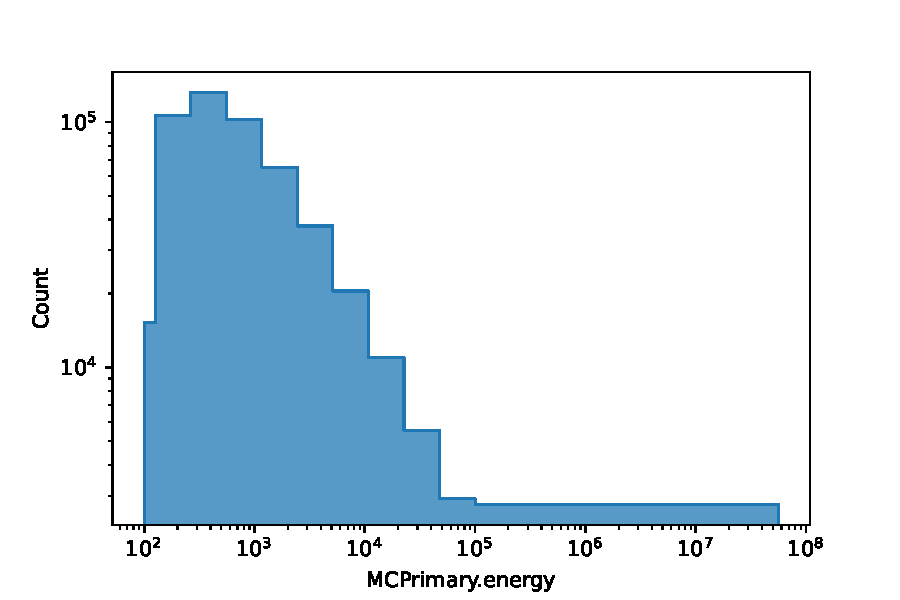
\includegraphics[width=0.5\textwidth]{content/plots/dataset:discretized:histogram.pdf}
  \caption{Energy spectrum of the 500k Monte-Carlo dataset using the discretized energy ranges as bins. TODO.}
  \label{fig:dataset:discretized:histogram}
\end{figure}


\subsection{Neural network}
\citeauthor{corn} provide a PyTorch \cite{pytorch} implementation of their \textsc{CORN} method
as well as several examples demonstrating its application on different datasets.
% TODO: Reference their tabular data / cement example?

This work makes use of said implementation of \textsc{CORN}
and hence the PyTorch framework.
Additionally,
  PyTorch Lightning \cite{pytorch_lightning},
  TorchMetrics \cite{torch_metrics}, % Oxford comma
  and scikit-learn \cite{sklearn}
  are used.

The neural network consists of \num{4} fully connected hidden layers.
The input layer has \num{12} neurons,
  corresponding to the number of features,
while the output layer has \num{9} neurons,
  corresponding to the number of binary classification subtasks,
    i.e. the number of bins minus one.
% \textsc{CORN} in the output layer…
% In total, the neural network has \num{TODO} neurons.

The number of neurons in the hidden layers is shown in \autoref{tab:nn_shape}.
\begin{itemize}
  \item Leaky ReLU activation function
  \item Fully connected layers
  \item Adam optimizer
\end{itemize}

\begin{table}
  \centering
  \caption{
    Shape and activation functions of the neural network.
    The number of neurons in the input and output layers is determined by the number of features and bins, respectively.
  }
  \label{tab:nn_shape}
  \begin{tabular}{S[table-format=3.0] c}
    \toprule
    {neurons} & {activation function} \\
    \midrule
    12  & – \\
    120 & leaky ReLU \\
    240 & leaky ReLU \\
    120 & leaky ReLU \\
    12  & leaky ReLU \\
    9   & leaky ReLU \\
    \bottomrule
  \end{tabular}
\end{table}

% TODO: Reference \textsc{CORN} loss function?

\emph{ADAM} (Adaptive Moment Estimation) \cite{adam} is used as the optimizer.
% It combines the benefits of both AdaGrad and RMSProp.

The neural network keeps its weights between \textsc{Dsea} iterations.
This was found to have no significant effect on the performance \cite{dsea_samuel}. % (\texttt{one\_model})


\subsection{DSEA}
For this work, the Python implementation of \textsc{Dsea} \cite{dsea_code} by \citeauthor{dsea_mirko} is used.
It expects a \emph{scikit-learn} classifier.
In order to interface with this library,
a wrapper class is implemented,
  which exposes a constructor as well as the needed methods
  \mintinline{python}{fit(X, y, sample_weight)} and
  \mintinline{python}{predict_proba(X)}.

  \section{Performance Metrics}
In order to evaluate the performance of the models
and to compare them to prior works,
several metrics are used.
%
For the calculation of all metrics that are mentioned here,
scikit-learn \cite{sklearn} is used.


\subsection{Accuracy} \label{sec:unfolding:metrics:accuracy}
The \emph{accuracy} \cite{accuracy} is the fraction of correctly classified events to the total number of events.
It is a common metric for classification tasks,
but it is not ideal for ordinal classification
  since it does not take the ordering of the classes into account.
For example,
the metric is the same for
a misclassification by one rank
and a misclassification by two ranks.
%
Nonetheless,
it gives an indication of the overall performance of the model.


\subsection{Mean Absolute Error} \label{sec:unfolding:metrics:mae}
% NOTE: Remember, ordinal classification ≙ ordinal regression.
The \acfi{MAE} \cite{mae} is a metric that is commonly used for regression tasks.
It is defined as
\begin{equation}
  \text{\acs{MAE}} = \frac{1}{N} \sum_{i=1}^N \left| y^{[i]} - \hat{y}^{[i]} \right|
\end{equation}
where $N$ is the number of events,
$y^{[i]}$ is the true value of the $i$-th event,
and $\hat{y}^{[i]}$ is the predicted value of the $i$-th event. % Oxford comma

% Because of its simple definition,
% it can be easily understood and interpreted.

Since the absolute value of the error is considered,
overestimation and underestimation are treated equally
and do not cancel each other out.
% NOTE: The referenced paper gives some good arguments for using MAE over RMSE.
In contrast to the \acfi{RMSE},
the \ac{MAE} is not especially sensitive to outliers
and has a more natural interpretation \cite{mae}.


\subsection{Wasserstein Distance} \label{sec:unfolding:metrics:wd}
The two previous metrics were based on single predictions for each event.
They disregard both
  the confidences of the predictions,
    considering only the prediction with the highest confidence,
  and the spectrum,
    which results from summing of the confidences over all events.

In contrast,
% NOTE: The cited paper calls it "Earth Mover's Distance", but I want the citation here for consistency.
the \emph{Wasserstein distance} \cite{wd}
compares the unfolded spectrum to the true spectrum.
%
It is also known as \acfi{EMD},
  hinting at the analogy of moving earth to transform one distribution into another,
    where the cost is given as the product of the distance and the amount of earth moved.
      % essentially the physical work.

Mathematically, the Wasserstein distance (of first kind) can be defined as
\begin{equation}
  \text{\acs{WD}}(\mathbf{p}, \mathbf{q}) = \inf_{\pi \in \Pi(\mathbf{p}, \mathbf{q})} \int_{\mathbb{R}^2} |x - y| \, \mathrm{d}\pi(x, y)
\end{equation}
where
  $\mathbf{p}$ and $\mathbf{q}$ are the probability distributions subject to comparison,
  $\Pi(\mathbf{p}, \mathbf{q})$ is the set of all probability distributions on $\mathbb{R}^2$,
  and $\pi$ is a probability distribution on $\mathbb{R}^2$.
% The Wasserstein distance is zero if and only if $\mathbf{p} = \mathbf{q}$.

  \section{Hyperparameters}
\subsection{Batch size}
The \emph{batch size} determines the number of events used for each training step.
While larger batch sizes increase the speed of training
on optimized hardware,
the quality of the local minima can be negatively affected.
% TODO: citation needed


\subsection{Adaptive step size: $J$-factor}
\begin{figure}
  \centering
  % TODO: correct dimensions
  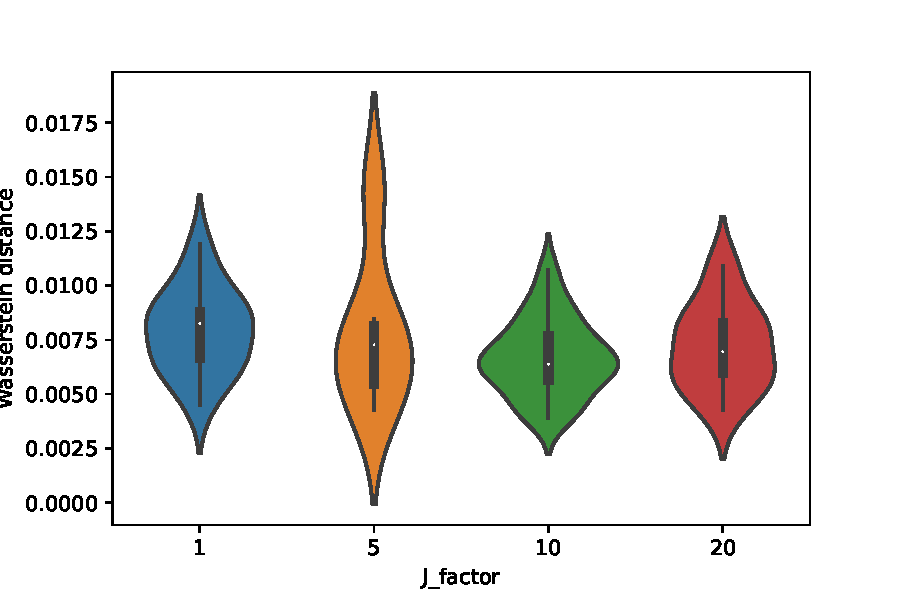
\includegraphics[scale=1]{content/plots/halftime/wd_per_J_factor.pdf}
  \caption{…}
  \label{fig:hyperparameter:J_factor}
\end{figure}

\subsection{Number of epochs}

  \section{Uncertainty and Results}
Using the best-performing hyperparameters from the hyperparameter search, % TODO: language
the final model is evaluated in more detail.
Specifically,
  the uncertainty of the predictions is analyzed, % Oxford comma
  and the physical plausibility of the predictions is investigated.


\subsection{Bootstrapping}
Bootstrapping \cite{bootstrap} is a method to estimate the uncertainty of a model.
It considers the given data as a random sample from a larger population.
Therefore,
by repeatedly sampling from the data and training a model on each sample,
the model's uncertainty can be determined
as the variance of the results of the different models.
%
For the present work, \num{50} bootstrap samples are used.
Since using a bootstrap sample of the same size as the original (\enquote{bag}) data set
might produce an inconsistent bootstrap estimator \cite{bootstrap_samplesize},
\num{1000000} events are used as the original data set,
while the bootstrap samples contain \num{500000} events as before.


\subsection{Energy Spectrum}
\todo{
  This is (probably) the most important plot. Discuss it in more detail!
}
\autoref{fig:bootstrap:spectrum} shows the unfolded energy spectrum of the optimized model,
as well as the \SI{68}{\percent} confidence intervals,
  ranging from the \SI{16}{\percent} to the \SI{84}{\percent} percentile.
In \autoref{fig:bootstrap:distributions},
the per-bin histograms of the estimations for individual bootstrap runs are shown.
While the probability density in the bins from \SI{E2}{\giga\electronvolt} to \SI{E4}{\giga\electronvolt} is estimated with high precision
  (relative deviation of \SI{6}{\percent} or less apart from the underflow bin),
both the relative deviation and the quantile range are large for the lower energy bins.
It can be speculated that this is due to the fact that the number of events in these bins is small in comparison,
which leads to a large uncertainty in the estimation of the spectrum.
% NOTE: Quadrupling the data set size did not help. :(

% TODO: more

\begin{figure}
  \centering
  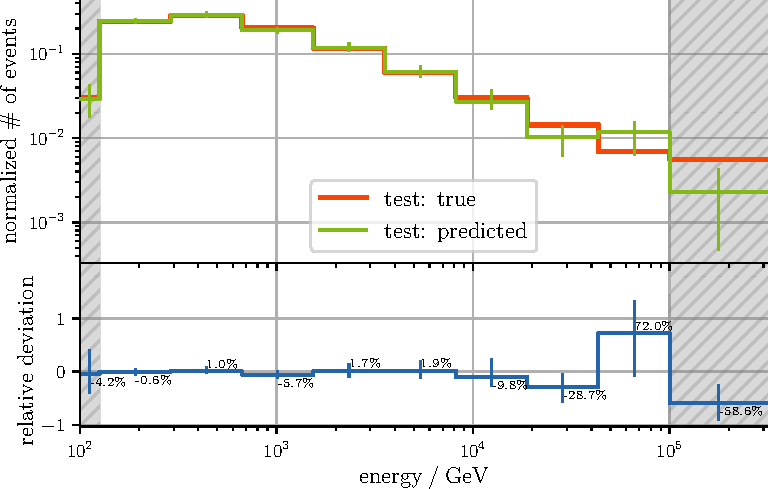
\includegraphics[scale=1]{content/plots/bootstrap:spectrum_full.pdf}
  \caption{
    Energy spectrum and relative deviations of the bootstrap.
    The error bars show the \SI{68}{\percent} confidence intervals,
    ranging from the \SI{16}{\percent} to the \SI{84}{\percent} percentile.
    The greyed out areas show the under- and overflow bins.
  }
  \label{fig:bootstrap:spectrum}
\end{figure}


\subsection{Individual Events}
Ordinal classification methods promise physically plausible results… % TODO
In contrast to \emph{LogisticAT},
    which \citeauthor{dsea_jan} used \cite{dsea_jan},
  the unimodality of the probability distribution is not enforced directly.
Instead,
  only the threshold probabilities ($f_k(\mathbf{x}^{[i]})$) are constrained to be monotonically increasing
  by the chain rule of probability
  (see \autoref{sec:corn:method}).
As can be seen in \autoref{fig:bootstrap:single_events},
  slight deviations from unimodality do occur.
Still,
  the indirect constraint on the threshold probabilities
  might be beneficial.

\begin{figure}
  \centering
  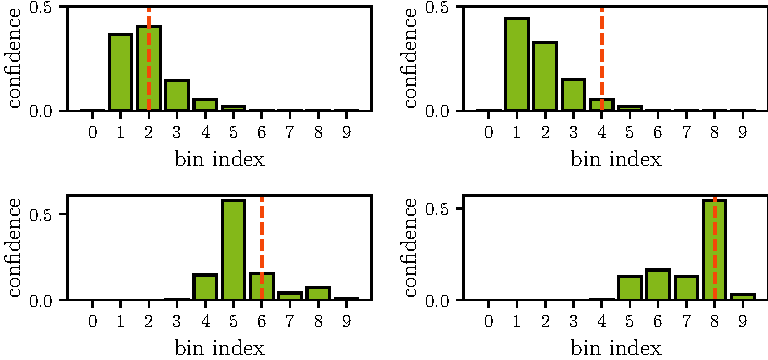
\includegraphics[scale=1]{content/plots/single_events_lessheight.pdf}
  \caption{
    Confidence distributions of selected events.
    The dashed orange line shows the true bin of the event.
    TODO: Find examples that violate the unimodality assumption.
  }
  \label{fig:bootstrap:single_events}
\end{figure}

% COULDDO: Compare to a Random Forest?

  \clearpage % guidance only
\section{Bias}
As explained in \autoref{sec:dsea:dsea},
\dsea{} is intended to eliminate the bias introduced by the energy spectrum of the Monte Carlo training data.
%
In order to test
whether the bias is indeed eliminated,
the model is trained on a \emph{stratified} dataset,
    where each bin contains an equal number of events.
The model is then evaluated on the unmodified dataset.
% TODO: explain that dataset(s): number of events etc.
% TODO: Make clear that train/test data don't overlap
% TODO: This is [if it were done…] the opposite of what I did earlier. But it matches what Samuel does. Both should be fine.

The results are shown in \autoref{fig:bias_comparison}.
As can be seen,
only a small bias remains:
The model adapts to the unseen distribution of the test data.
… in comparison to \autoref{fig:bootstrap:spectrum}.

In the work by \citeauthor{dsea_samuel},
relative deviations of more than \SI{1500}{\percent} are observed \cite{dsea_samuel}.
% Aber er schiebt's auf die geringe Accuracy…


\begin{figure}[H]
    \centering
    \begin{subfigure}{0.45\textwidth}
        \centering
        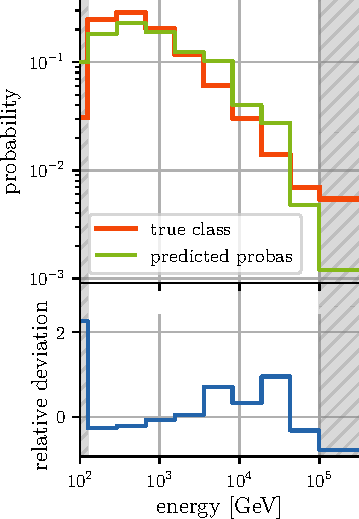
\includegraphics[width=\textwidth]{content/plots/bootstrap:spectrum_halfwidth.pdf}
        \caption{
            Placeholder for spectrum A.
            There is bias. Blah.
        }
        % \label{fig:TODO}
    \end{subfigure}
    \begin{subfigure}{0.45\textwidth}
        \centering
        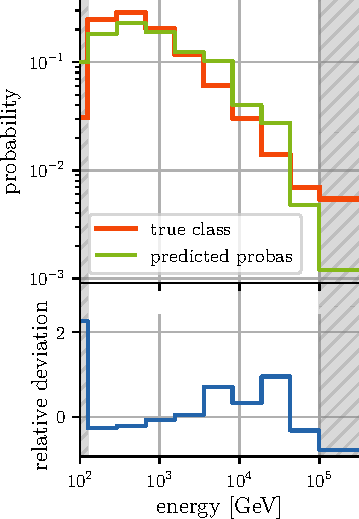
\includegraphics[width=\textwidth]{content/plots/bootstrap:spectrum_halfwidth.pdf}
        \caption{
            Placeholder for spectrum B.
            There is no bias. Blah.
        }
        % \label{fig:TODO}
    \end{subfigure}
    \caption{
        Comparison of…
        Lorem ipsum dolor sit amet, consectetur adipiscing elit.
    }
    \label{fig:bias_comparison}
\end{figure}

\chapter{Summary and Outlook} \label{sec:summary}
% should be 1 page

% █ What did I achieve?
It has been shown that
the combination of neural networks, ordinality and \dsea{}
  can be successfully applied to
  the problem of neutrino energy spectrum estimation
  with \icecube{} data.
This was enabled by
  adding support for
    sample weights
    and confidences
  to \ac{CORN}.

% █ comparisons
The new method is not unambiguously superior to the previous ones
  (\cite{dsea_jan} and \cite{dsea_samuel}).
A strict comparison is not possible
    in the first place,
  as this work introduces under-/overflow bins
  and makes use of adaptive step sizes.
% 1. confidence distributions → Samuel
The randomly selected confidence distributions of a common neural network using softmax \cite{dsea_samuel}
  are of comparable quality to those obtained in this work (see \autoref{fig:bootstrap:single_events}),
    even though ordinality is disregarded in the former case.
  % Compared to the confidence distributions of \emph{LogisticAT} \cite{dsea_jan}, …
%
% 2. accuracy → Samuel
Compared to \cite{dsea_samuel},
  higher \hyperref[sec:unfolding:metrics:accuracy]{accuracy} is achieved
    (ours: \SI{42.7}{\percent} vs. theirs: $< \SI{39}{\percent}$).
Both the \ac{RMSE}
  (\num{0.0164} vs. \num{0.000269})
and the $\chi^2$ distance
  (\num{0.0392} vs. \num{0.003123})
are worse,
  however,
because of the large deviations in higher energy bins.
%
% 3. Wasserstein distance → Jan
In comparison to \cite{dsea_jan},
  similar \hyperref[sec:unfolding:metrics:wd]{Wasserstein distances} are achieved
    (\num{0.0108} vs. \num{0.00879}),
    but using \num{10} instead of \num{12} bins.
On the other hand,
our probability distributions of single events are not strictly unimodal.


% █ future work
There is still a multitude of ways in which \dsea{} and the application thereof could be improved.
%
Explicit \hyperref[sec:dsea:deconvolution_problem:regularization]{regularization}
could dampen the currently observed oscillations in higher energy bins.
%
Other hyperparameters,
  such as the shape of the neural network,
are yet to be optimized.
%
It might be possible to modify \ac{CORN}
  so that the per-class confidence distributions are strictly unimodal.
In general,
other neural network architectures
  could be investigated.
For example,
  graph neural networks
  already exceed boosted decision trees
    in terms of both resolution and speed \cite{minh2021gnn}.
%
Graph neural networks
have the additional benefit of
being less dependent on feature engineering
  as they can be applied to \enquote{raw} data
    (%
      which \ac{DOM} was hit,
      the collected charge, % Oxford comma
      and the time of arrival%
    ).
%
Finally,
  more data could be used for training.
Because of the shape of the spectrum,
  the number of events in the highest energy bins
  remains relatively small
    compared to the complete data set.
Although this thesis has \hyperref[sec:unfolding:bias]{demonstrated that \dsea{} eliminates the training bias},
  the effect of stratified training data on the overall performance
  has not been investigated.
% NOTE: We can't stratify the real-world data, only the training data.


% COULDDO:
% \section{(Comparison to Conventional Neural Networks)}
% \section{(Comparison to LogisticAT)}



  \appendix
  % Hier beginnt der Anhang, nummeriert in lateinischen Buchstaben
  \chapter{Appendix}

\section{Detector Signatures of Different Neutrino Flavors}
\begin{figure}
  \centering
  \begin{subfigure}{0.3\textwidth}
    \centering
    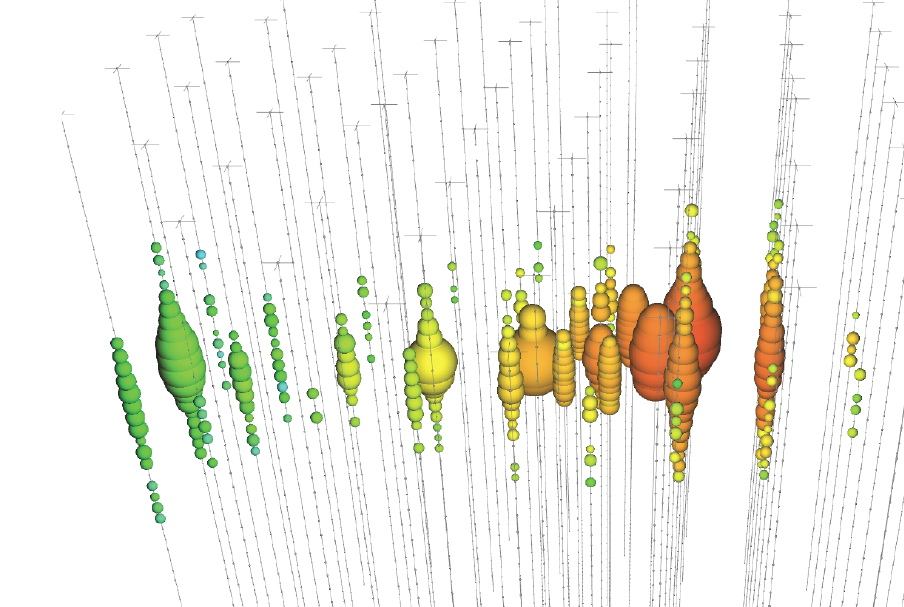
\includegraphics[width=\textwidth]{content/img/signatures/track.png}
    \caption{
        Track / $\nu_\mu$
    }
  \end{subfigure}
  \begin{subfigure}{0.3\textwidth}
    \centering
    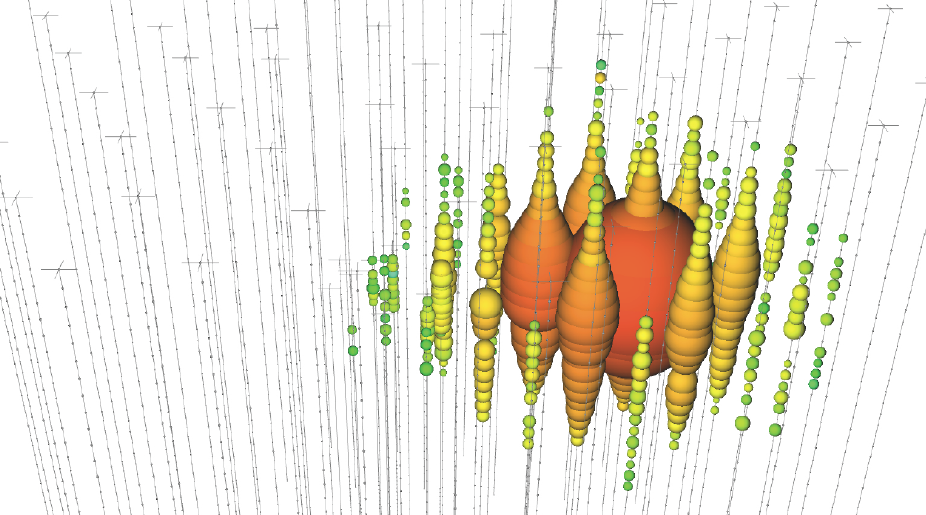
\includegraphics[width=\textwidth]{content/img/signatures/cascade.png}
    \caption{
        Cascade / $\nu_e$
    }
  \end{subfigure}
  \begin{subfigure}{0.3\textwidth}
    \centering
    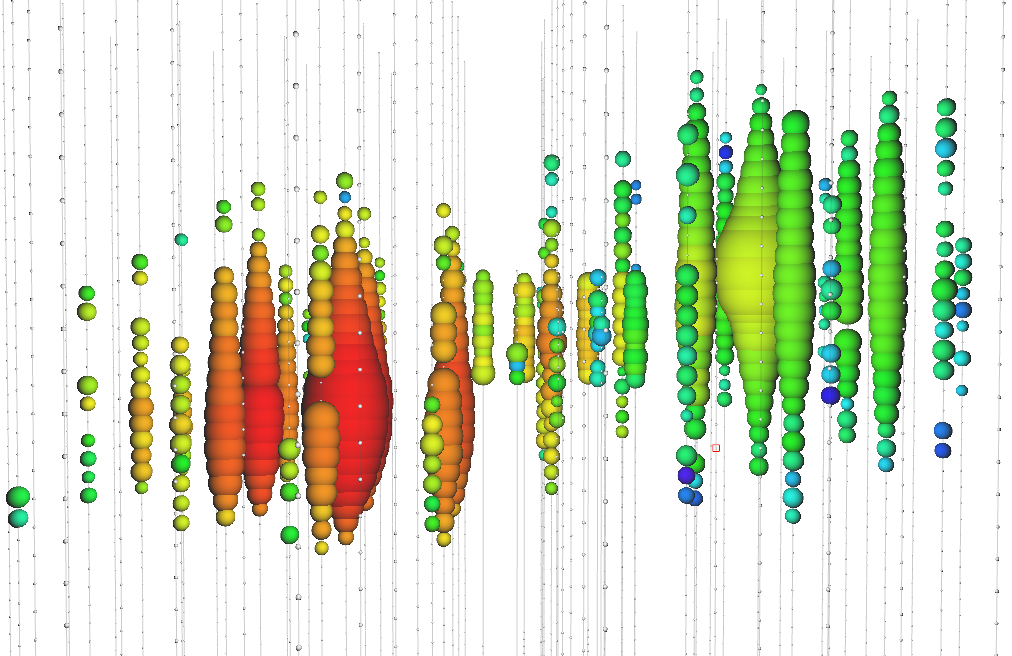
\includegraphics[width=\textwidth]{content/img/signatures/double_bang.png}
    \caption{
        Double bang / $\nu_\tau$
    }
  \end{subfigure}
  \caption{
    Shapes of the Cherenkov light produced by neutrinos of different flavors.
    The coloring of the \textsc{Dom}s indicates the time of the interaction,
    with red being the earliest and blue being the latest.
    \cite{kowalski2017} % CC-BY 3.0
  }
  \label{fig:img:icecube:interactions}
\end{figure}


\clearpage
\section{\texorpdfstring{$\text{DSEA}^+$}{DSEA+}: Complete Algorithm} \label{sec:alg:dseaplus}
\begin{algorithm}
  \caption{
    The \dseaplus{} algorithm with reweighting of training examples and adjustable stepsize. \cite{dsea_mirko}
    \todo[inline]{
      This is taken 1:1 from Mirko's thesis.
      I didn't quite get @Karolin's feedback on this:
      Should I remove it?
      }
    }
  \label{alg:dseaplus}
  \begin{algorithmic}
    \newcommand{\f}{\mathbf{f}}
    \newcommand{\hatf}{\hat{\mathbf{f}}}
    \newcommand{\x}{\mathbf{x}}

    \Require{
      \\
      Observed data set $\mathcal{D}_\text{obs} = \{ \x_n \in \mathcal{X} : 1 \leq n \leq N \}$ \\
      Training data set $\mathcal{D}_\text{test} = \{ (\x_n, y_n) \in \mathcal{X} \times \{1,\ldots,I\} : 1 \leq n \leq N' \}$ \\
      $\tau \geq 0$, regularization strength employed in the stepsize adaptation (default: \num{0}) \\
      $\epsilon > 0$, the minimal $\chi_\text{Sym}^2$ distance between subsequent iterations (default: \num{E-6}) \\
      Prior density $\hatf^{(0)}$ (default: $\hatf_i^{(0)} = \frac{1}{I} \forall 1 \leq j \leq J$)
    }
    \Ensure Estimated target density $\hatf \in \mathbb{R}^I$
    \State $k \gets 0$
    \Repeat
      \State $k \gets k-1$\;
      \State $\forall 1 \leq n \leq N': w_n^{(k)} \gets \hatf_{i (n)}^{(k-1)} / \f_{i (n)}^t$\;
      \State Infer $\mathcal{M}$ from $\mathcal{D}_\text{train}$ weighted by $w_n^{(k)+}$\;
      \State $\forall 1 \leq i \leq I: p_i^{(k)} \gets \frac{1}{N} \sum_{n=1}^N c_{\mathcal{M}}(i|\x_n) - \hatf^{(k-1)}$\;
      \State $\alpha_{\textsc{Run}}^{(k)} \gets \operatorname{argmin}_{\alpha \geq 0} \ell_r(\hatf^{(k-1)} + \alpha p^{(k)})$\;
      \State $\hatf_i^{(k)+} \gets \hatf^{(k-1)} + \alpha_{\textsc{Run}}^{(k)} \cdot p^{(k)}$\;
    \Until $\chi_\text{Sym}^2(\hatf^{(k)}, \hatf^{(k-1)}) \leq \epsilon$\; \\
    \Return $\hatf \gets \hatf^{(k)}$
  \end{algorithmic}
\end{algorithm}



\clearpage
\section{From Threshold to Per-Class Probabilities}
\label{sec:appendix:corn_probas}
Given four ranks with indices $q \in \{1, 2, 3, 4\}$,
\corn{}'s output layer has three neurons, which
  – after applying sigmoid and a cumulative product –
yield three threshold probabilities:
	$P[q>1]$,
	$P[q>2]$ and
	$P[q>3]$.
The goal is to calculate the probability of each class $q$,
i.e. $P[q=1]$, $P[q=2]$, $P[q=3]$ and $P[q=4]$.

% The solution explicitly requires the assumption that…
Using $q \in \{1, 2, 3, 4\}$,
the following equations hold:
\begin{align*}
  P[q=1] &= \neg P[q>1] = 1 - P[q>1] \\
  \\
  P[q=2] &= \neg P[q≠2] \\
  &= \neg(P[q<2] \lor P[q>2]) \\
  &= 1 - ((1 - P[q>1]) + P[q>2]) \\
  &= P[q>1] - P[q>2] \\
  \\
  P[q=3] &= \neg P[q≠3] \\
  &= \neg(P[q<3] \lor P[q>3]) \\
  &= 1 - ((1 - P[q>2]) + P[q>3]) \\
  &= P[q>2] - P[q>3] \\
  \\
  P[q=4] &= P[q>3] \, .
\end{align*}

The same principle can be applied to any number of classes.


\clearpage
\section{Monte Carlo Dataset}
\begin{figure}
  \centering
  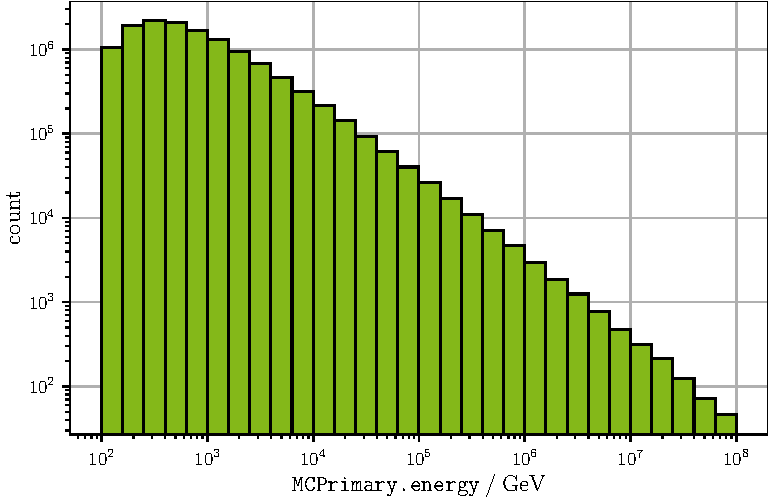
\includegraphics[scale=1]{content/plots/dataset:raw:histogram_full.pdf}
  \caption{Energy spectrum of the full, untouched Monte Carlo dataset using 30 bins.}
  \label{fig:dataset:raw:histogram}
\end{figure}


\clearpage
\section{Additional Hyperparameter Plots}
\begin{figure}
  \centering
  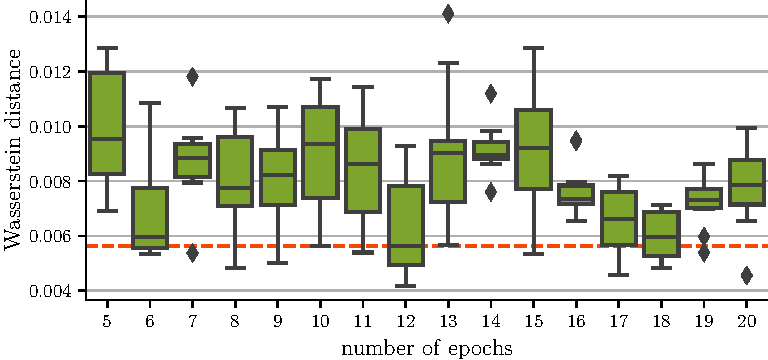
\includegraphics[scale=1]{content/plots/hyperparam/num_epochs_vs_wd_boxplot_lessheight.pdf}
  \caption{Boxplot of the accuracy for different epoch counts.}
  \label{fig:hyperparameter:num_epochs_vs_wd_boxplot}
\end{figure}

% COULDDO: add more?

\clearpage
\section{Bootstrap Distributions}
\begin{figure}
  \centering
  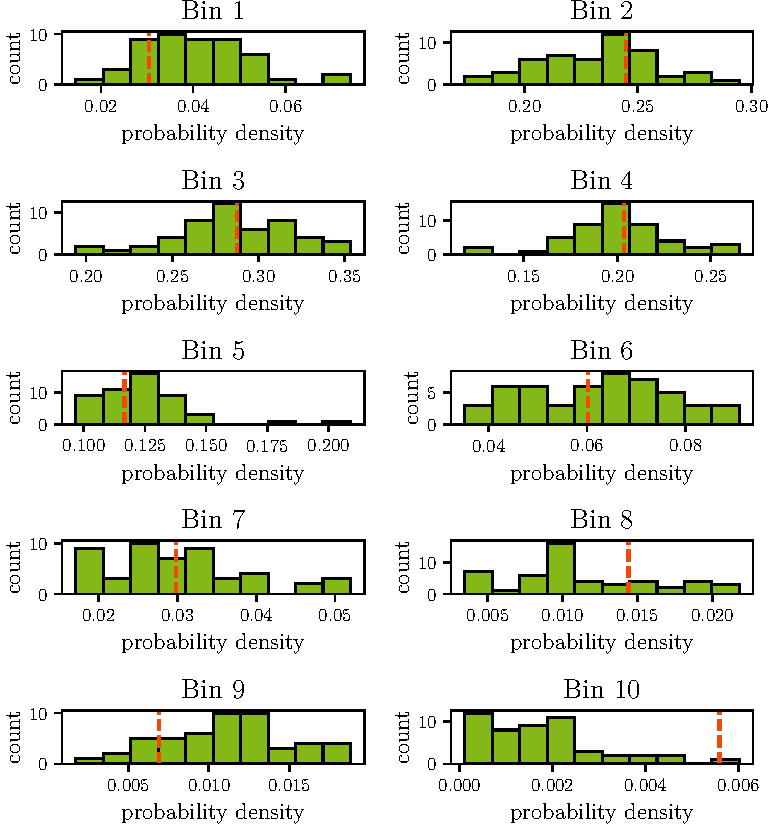
\includegraphics[scale=1]{content/plots/bootstrap:distributions_doubleheight.pdf}
  \caption{
    Bootstrap distributions of each bin in \autoref{fig:bootstrap:spectrum}.
    The dashed orange line shows the true value.
  }
  \label{fig:bootstrap:distributions}
\end{figure}


\clearpage
\section{Links etc.}
\begin{description}
  \item[Code on the chair's GitLab] \hfill \\
    \url{https://git.e5.physik.tu-dortmund.de/nweitkemper/Bachelor-code}
  \item[Dataset in the chair's \texttt{POOL} file system] \hfill \\
    \texttt{/net/big-tank/POOL/users/lkardum/new\_mc\_binning.csv} (\SI{14.6}{\giga\byte})
  % https://git.e5.physik.tu-dortmund.de/shaefs/bachelor_thesis/
\end{description}


  \backmatter
  \printbibliography

  \chapter*{Acknowledgements}

Thanks to
  Prof.~Dr.~Dr.~Wolfgang~Rhode and
  Prof.~Dr.~Johannes~Albrecht
  for taking the time to review my thesis
  and for being open to questions.

I would also like to thank
my supervisors
  Karolin~Hymon and
  Leonora~Kardum
as well as
  Tim~Ruhe and
  Mirko~Bunse
for their support and guidance throughout this project.

Furthermore,
I am grateful to Samuel~Haefs,
  who worked on his Bachelor's thesis in parallel with me,
for the inspiring discussions
and for providing a baseline for the implementation of neural networks in \dsea{}.

I appreciate the chair~E5b providing
  the technical infrastructure
  and helpful feedback
    regarding my half-time talk.

% NOTE: Nöthe → Linhoff
Thanks to Dr.~Maximilian~Linhoff for providing a \href{https://github.com/maxnoe/tudothesis}{\LaTeX{} template} for this thesis.

A special thanks to my family for their continued support and encouragement.


  \cleardoublepage
  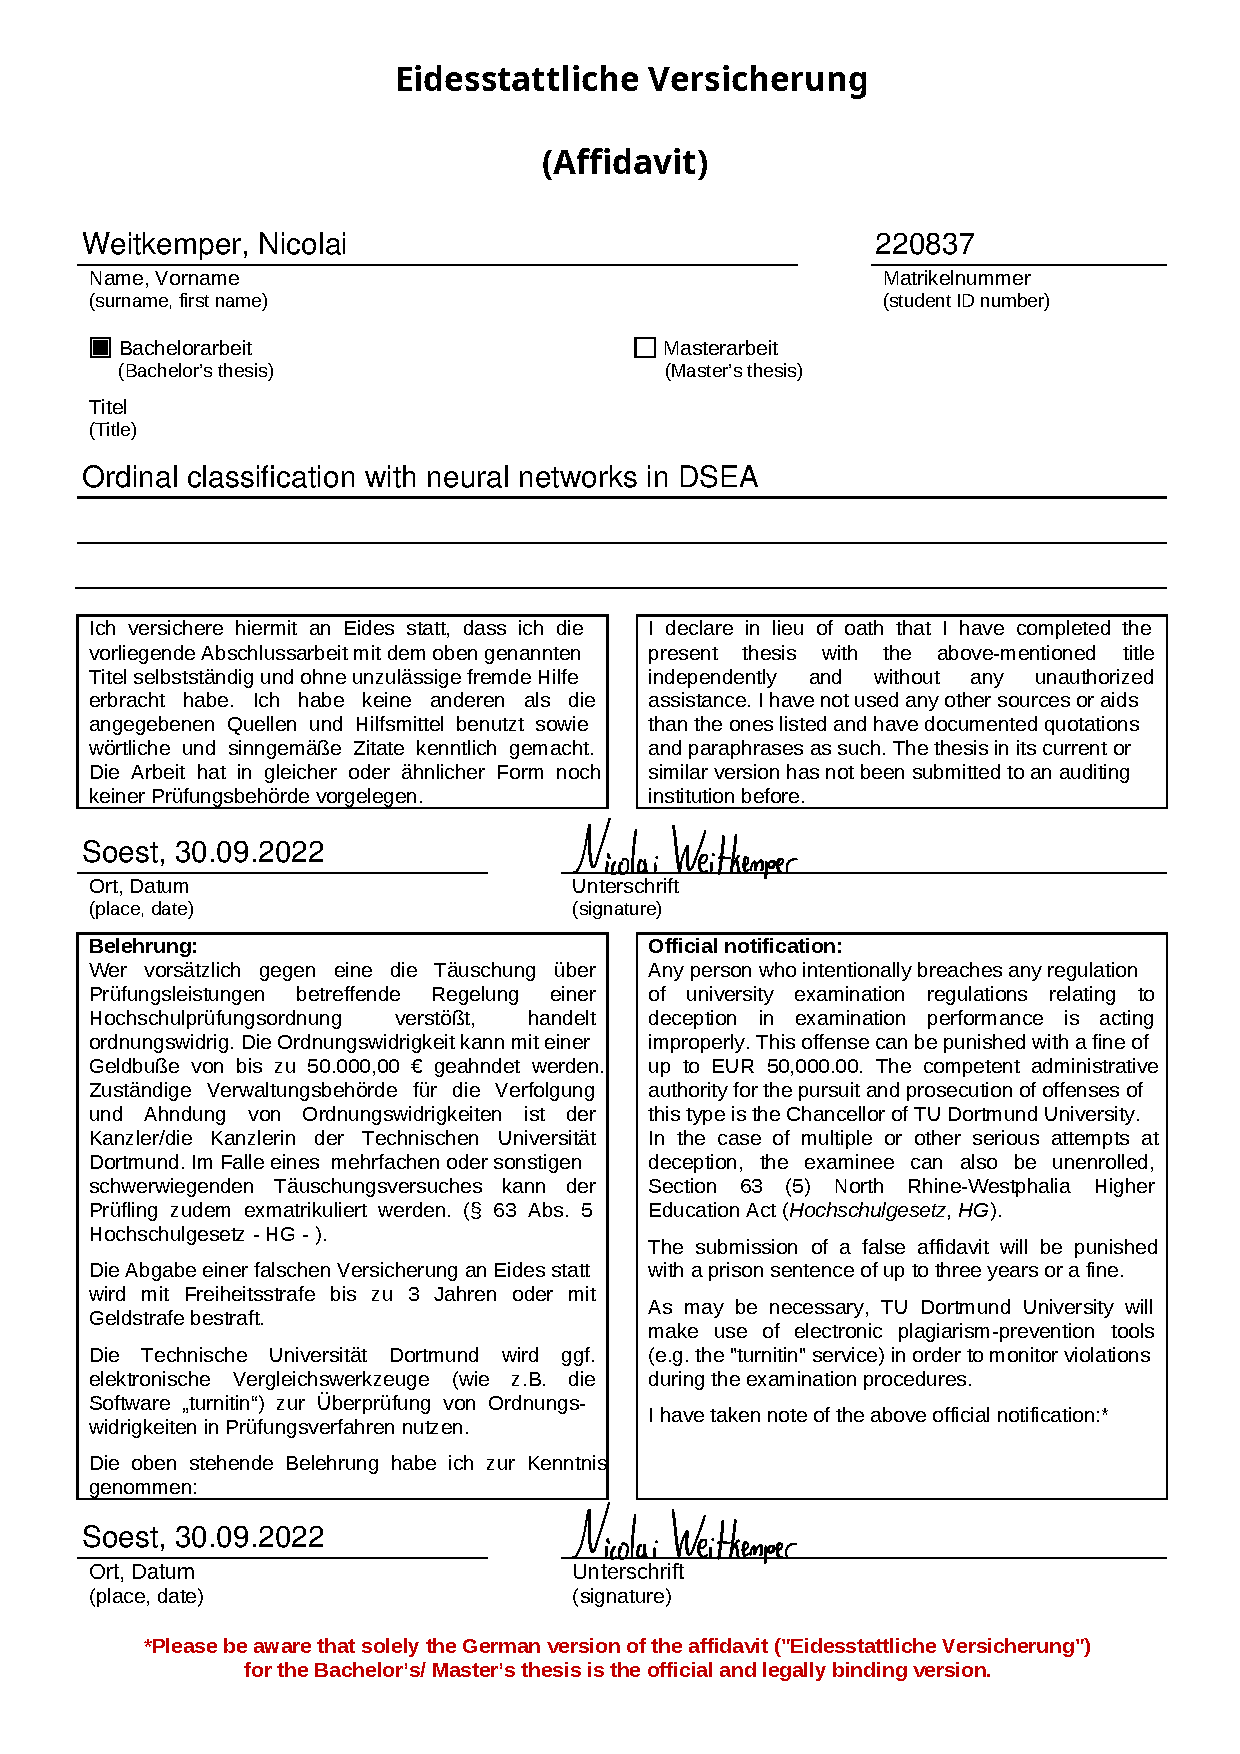
\includepdf[pages=-]{content/affidavit.pdf}
\end{document}
